\documentclass[letterpaper,12pt]{article}
\usepackage{array}
\usepackage{threeparttable}
\usepackage{geometry}
\geometry{letterpaper,tmargin=1in,bmargin=1in,lmargin=1.25in,rmargin=1.25in}
\usepackage{fancyhdr,lastpage}
\pagestyle{fancy}
\lhead{}
\chead{}
\rhead{}
\lfoot{}
\cfoot{}
\rfoot{\footnotesize\textsl{Page \thepage\ of \pageref{LastPage}}}
\renewcommand\headrulewidth{0pt}
\renewcommand\footrulewidth{0pt}
\usepackage[format=hang,font=normalsize,labelfont=bf]{caption}
\usepackage{listings}
\lstset{frame=single,
  language=Python,
  showstringspaces=false,
  columns=flexible,
  basicstyle={\small\ttfamily},
  numbers=none,
  breaklines=true,
  breakatwhitespace=true
  tabsize=3
}
\usepackage{amsmath}
\usepackage{amssymb}
\usepackage{amsthm}
% \usepackage{harvard}
\usepackage{setspace}
\usepackage{float,color}
\usepackage[pdftex]{graphicx}
\usepackage{hyperref}
\hypersetup{colorlinks,linkcolor=red,urlcolor=blue}
\theoremstyle{definition}
\newtheorem{theorem}{Theorem}
\newtheorem{acknowledgement}[theorem]{Acknowledgement}
\newtheorem{algorithm}[theorem]{Algorithm}
\newtheorem{axiom}[theorem]{Axiom}
\newtheorem{case}[theorem]{Case}
\newtheorem{claim}[theorem]{Claim}
\newtheorem{conclusion}[theorem]{Conclusion}
\newtheorem{condition}[theorem]{Condition}
\newtheorem{conjecture}[theorem]{Conjecture}
\newtheorem{corollary}[theorem]{Corollary}
\newtheorem{criterion}[theorem]{Criterion}
\newtheorem{definition}[theorem]{Definition}
\newtheorem{derivation}{Derivation} % Number derivations on their own
\newtheorem{example}[theorem]{Example}
\newtheorem{exercise}[theorem]{Exercise}
\newtheorem{lemma}[theorem]{Lemma}
\newtheorem{notation}[theorem]{Notation}
\newtheorem{problem}[theorem]{Problem}
\newtheorem{proposition}{Proposition} % Number propositions on their own
\newtheorem{remark}[theorem]{Remark}
\newtheorem{solution}[theorem]{Solution}
\newtheorem{summary}[theorem]{Summary}
%\numberwithin{equation}{section}
\bibliographystyle{aer}
\newcommand\ve{\varepsilon}
\newcommand\boldline{\arrayrulewidth{1pt}\hline}

\begin{document}
\begin{flushleft}
  \textbf{\large{Problem Set \#2}} \\
  MACS 30100, Dr. Evans \\
  Sushmita V Gopalan
\end{flushleft}

\vspace{5mm}
\noindent\textbf{Part 1(a).} 

\begin{figure}[htb]\centering\captionsetup{width=4.0in}
  \fbox{\resizebox{4.0in}{3.0in}{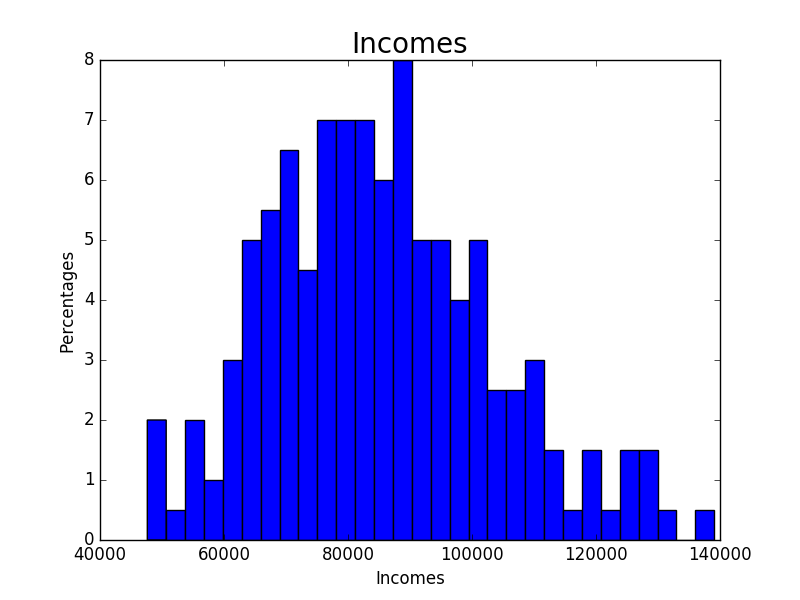
\includegraphics{Histogram.png}}}
\end{figure}
\vspace{5mm} %5mm vertical space
\noindent\textbf{Part 1(b).} 
\newline Log likelihood =  -8298.63695601

\begin{figure}[htb]\centering\captionsetup{width=4.0in}
 \fbox{\resizebox{4.0in}{3.0in}{\includegraphics{First_PDF.png}}}
\end{figure}
\vspace{20mm} %5mm vertical space

\noindent\textbf{Part 1(c).} 

\begin{figure}[htb]\centering\captionsetup{width=4.0in}
 \fbox{\resizebox{4.0in}{3.0in}{\includegraphics{Second_PDF.png}}}
\end{figure}

MLE mean =  11.3314403301 
\newline MLE sigma =  0.211674583829
\newline Log likelihood function value:  -2239.534744
\newline Variance/Covarience Matrix: 
\newline
 [ 0.00014668  0.00017025]
\newline
 [ 0.00017025  0.00030278]
 
\vspace{5mm} %5mm vertical space

\noindent\textbf{Part 1(d).} \newline chi squared of H0 with 2 degrees of freedom p-value =  0.0
\newline
We can reject the null hypothesis.
\vspace{5mm} %5mm vertical space

\noindent\textbf{Part 1(e).}
\newline Percentage of students will earn more than 100,000:  19.58%
\newline Percentage of students will earn less than 75,000:  30.77%

\vspace{5mm} %5mm vertical space

\noindent\textbf{Part 1(e).}
\newline Percentage of students will earn more than 100,000:  19.58%
\newline Percentage of students will earn less than 75,000:  30.77%

\vspace{5mm} %5mm vertical space

\noindent\textbf{Part 2(a).} 
\newline Beta0 = 0.252015425596  
\newline Beta1 = 0.0129518865934 
\newline Beta2 = 0.400302306248 
\newline Beta3 = -0.0100091666596 
\newline Sigma = 0.0518140029396
\vspace{20mm} %5mm vertical space

The variance-covariance matrix is: 
 \newline [ 1.  0.  0.  0.  0.]
 \newline [ 0.  1.  0.  0.  0.]
 \newline [ 0.  0.  1.  0.  0.]
 \newline [ 0.  0.  0.  1.  0.]
 \newline [ 0.  0.  0.  0.  1.]

Log-likelihood:  407.89171935524257

\noindent\textbf{Part 2(b).} 
\newline chi squared of H0 with 5 degrees of freedom p-value = 0.0
\newline We can reject the hypothesis that age, average temperature and number of children have no effect on sick days


\end{document}